%%%%%%%%%%%%%%%%%%%%%%%%%%%%%%%%%%%%%%%%%
% University Assignment Title Page 
% LaTeX Template
% Version 1.0 (27/12/12)
%
% This template has been downloaded from:
% http://www.LaTeXTemplates.com
%
% Original author:
% WikiBooks (http://en.wikibooks.org/wiki/LaTeX/Title_Creation)
%
% License:
% CC BY-NC-SA 3.0 (http://creativecommons.org/licenses/by-nc-sa/3.0/)
% 
% Instructions for using this template:
% This title page is capable of being compiled as is. This is not useful for 
% including it in another document. To do this, you have two options: 
%
% 1) Copy/paste everything between \begin{document} and \end{document} 
% starting at \begin{titlepage} and paste this into another LaTeX file where you 
% want your title page.
% OR
% 2) Remove everything outside the \begin{titlepage} and \end{titlepage} and 
% move this file to the same directory as the LaTeX file you wish to add it to. 
% Then add \input{./title_page_1.tex} to your LaTeX file where you want your
% title page.
%
%%%%%%%%%%%%%%%%%%%%%%%%%%%%%%%%%%%%%%%%%
%\title{Title page with logo}
%----------------------------------------------------------------------------------------
%	PACKAGES AND OTHER DOCUMENT CONFIGURATIONS
%----------------------------------------------------------------------------------------

\documentclass[12pt]{article}
\usepackage[utf8]{inputenc}
\usepackage[brazil]{babel}
\usepackage{amsmath}
\usepackage{amssymb}
\usepackage{graphicx}
\usepackage[colorinlistoftodos]{todonotes}
\usepackage{enumitem}
\usepackage{subcaption}
\usepackage{geometry}
    \geometry{
    a4paper,
    total={170mm,257mm},
    left=20mm,
    top=20mm,
    }
\usepackage[document]{ragged2e}
\usepackage[toc,page]{appendix}
\usepackage[framed,numbered,autolinebreaks,useliterate]{mcode}
\usepackage{float}

\newcommand{\HRule}{\rule{\linewidth}{0.5mm}} % Defines a new command for the horizontal lines, change thickness here
\renewcommand\appendixpagename{Apêndice: Identidades trigonométricas}

\begin{document}
%----------------------------------------------------------------------------------------
%	HEADING SECTIONS
%----------------------------------------------------------------------------------------

\begin{minipage}{0.15\textwidth}
    \begin{flushleft}
        
\includegraphics[width=\linewidth]{logo.png}
    \end{flushleft}
\end{minipage}
~
\begin{minipage}{0.75\textwidth}
    \textsc{Universidade de São Paulo}\\
    \textsc{Escola de Engenharia de São Carlos}\\
    \textsc{Departamento de Engenharia Elétrica e de Computação}\\
    \textsc{\textbf{SEL0343 | Processamento Digital de Sinais}}\\
    \textsc{\textbf{Prof. Dr. Emiliano R. Martins}}
\end{minipage}

\begin{flushright}
    {\small \today}
\end{flushright}

%----------------------------------------------------------------------------------------
%	AUTHOR SECTION
%----------------------------------------------------------------------------------------

\begin{minipage}{0.52\textwidth}
\begin{flushleft} \large
\emph{Aluno:}\\
\textbf{Luís Filipe Vasconcelos Peres} % Your name
\end{flushleft}
\end{minipage}
~
\begin{minipage}{0.45\textwidth}
\begin{flushright} \large
\emph{Nº USP:} \\
\textbf{10310641} % Supervisor's Name
\end{flushright}
\end{minipage}\\

%----------------------------------------------------------------------------------------
%	TITLE SECTION
%----------------------------------------------------------------------------------------
\center
\HRule \\[0.4cm]
{ \LARGE \bfseries Prova única}\\ % Title of your document
\HRule \\[0.2cm]

%----------------------------------------------------------------------------------------
%	CONTENT SECTION
%----------------------------------------------------------------------------------------
\justify
\section*{Problemas}
\section{}

Para a onda PM, temos:

\begin{align*}
    s (t) &= A_c \cdot \cos\theta_i\\
    \theta_i (t) &= k_p \cdot m(t) + 2\pi t f_c
\end{align*}

A frequência instantânea é dada por:

$$
    f_i(t) = f_c + A\cdot\left[ \frac{k_p}{2\pi T_0}
    - \sum_n \frac{k_p}{2\pi} \cdot \delta(t - nT_0)\right]
$$

Analisando a equação, obtemos que o valor da frequência será dado por (\ref{eq:freq}), porém com um deslocamento de fase (dado por (\ref{eq:pshift})) nos pontos de descontinuidade do sinal.

\begin{align}\label{eq:freq}
    f_i (t) = f_c + \frac{A\cdot k_p}{2\pi T_0}
\end{align}
\begin{align}\label{eq:pshift}
    \phi = \frac{-A \cdot k_p}{T_0}
\end{align}

Já para a onda FM, não vemos as mesmas descontinuidades:

\begin{align*}
    f_i (t) = k_f \cdot m(t) + f_c
\end{align*}

\begin{figure}[H]
    \begin{minipage}{0.5\textwidth}
        \centering
        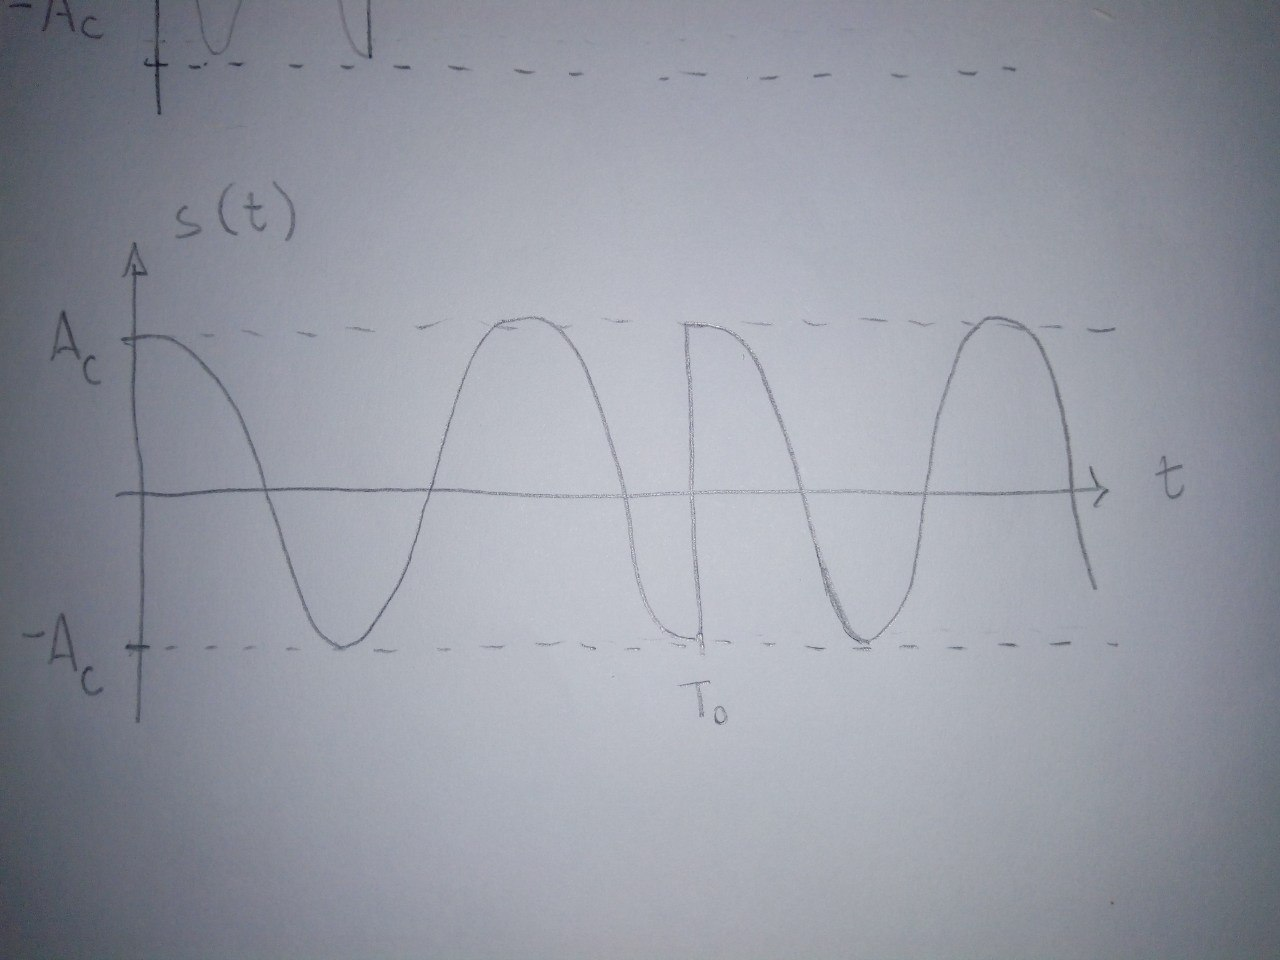
\includegraphics[width=0.9\linewidth]{phase.jpg}
        \caption{Esboço da onda PM produzida pela rampa.}
        \label{fig:my_label}
    \end{minipage}%
    \begin{minipage}{0.5\textwidth}
        \centering
        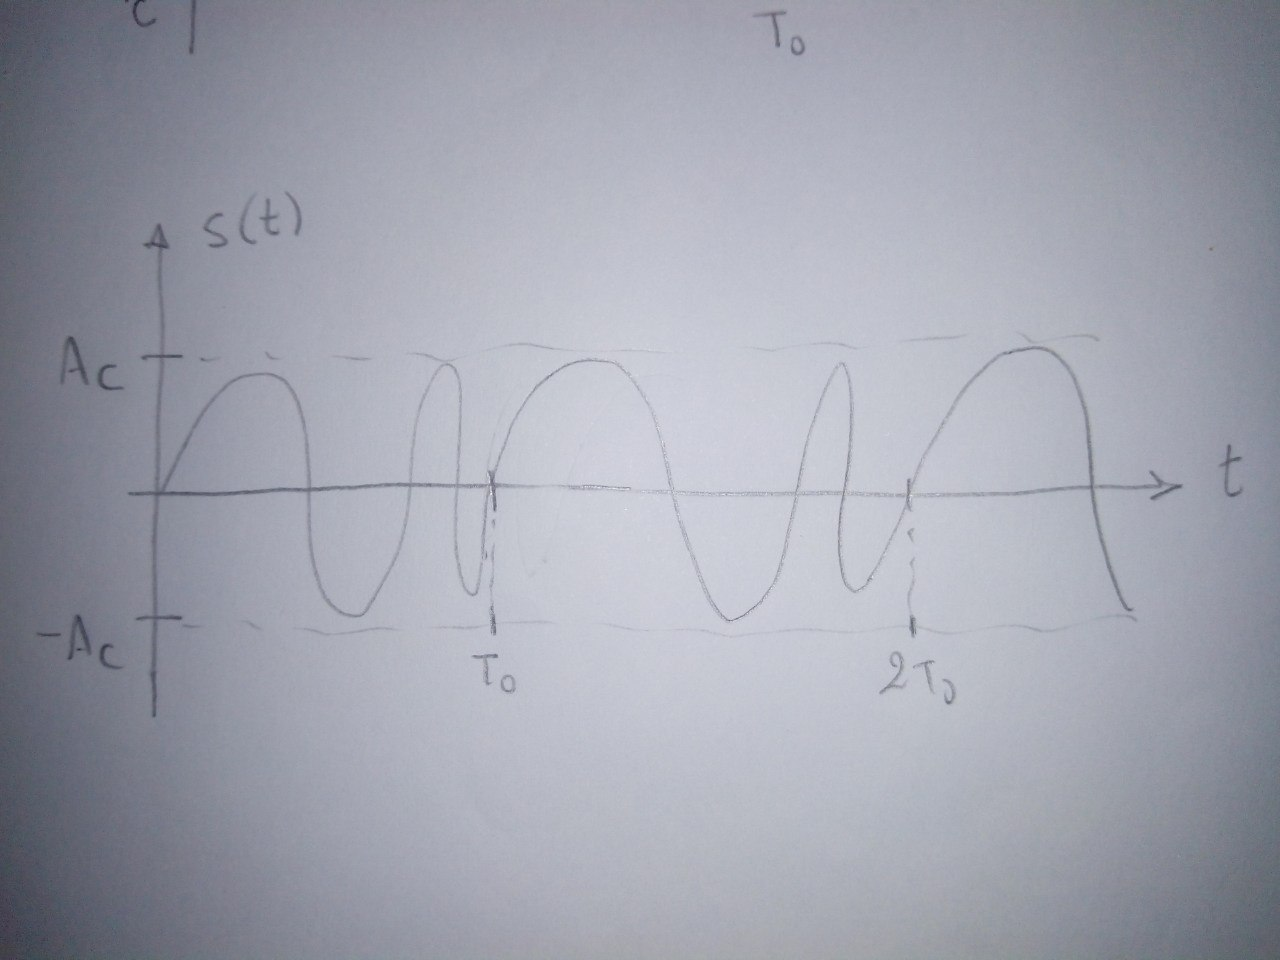
\includegraphics[width=0.9\linewidth]{frequency.jpg}
        \caption{Esboço da onda FM produzida pela rampa.}
        \label{fig:my_label}
    \end{minipage}
\end{figure}

\section{}

Determinando $s_n(t)$:
\begin{align*}
    s_n (t) &= a \cdot (J_0\cdot \cos(2\pi f_c t) \\
    &+ J_1 \cdot [\cos(2\pi t \cdot [f_c + f_m]) - \cos(2\pi t \cdot [f_c - f_m])]\\
    &+ J_2 \cdot [\cos(2\pi t \cdot [f_c + 2 f_m]) - \cos(2\pi t \cdot [f_c - 2 f_m])])
\end{align*}

Sabendo que $\beta = 1$, temos as funções de Bessel $J_n(\beta)$:
\begin{align*}
    J_0 (1) &= 0.765\\
    J_1 (1) &= 0.44\\
    J_2 (1) &= 0.115
\end{align*}

Com as funções de Bessel, com a expressão para $s_n$ supondo $A=1$, e conhecendo freq. banda média, largura de banda, freqs. de portadora e da onda modulante, usando as identidades trigonométricas do apêndice, temos o \textbf{espectro}:

\begin{align*}
    f_c - 2f_m &= 0.058\\
    f_c - fm &= 0.22\\
    f_c &= 0.382\\
    f_c + f_m &= 0.22\\
    f_c + 2fm &= 0.058
\end{align*}

\section{}
\paragraph{(a)}

Sabemos que:
\begin{align*}
    \Delta f &= k_f \cdot A_m\\
    \beta &= \frac{\Delta f}{f_m}
\end{align*}

Podemos obter que desvio de frequência será: 
$$
    \Delta f = 25 \cdot 10^3 \cdot 20 = 5 \cdot 10^5 = 500 kHz
$$
E para o índice de modulação:
$$
    \beta = \frac{5 \cdot 10^5}{10^5} = 5
$$

A partir da regra de Carson temos que $B_T = 2f_m(1+\beta)$, ou seja:
$$
    BW = 2\cdot 100 \cdot (1 + 5) = 1,2 \cdot 10^6 = 1,2 MHz
$$

\paragraph{(b)}
Sabendo que $\beta = 5$ temos que $\frac{BW}{\Delta f} = 3$. Assim, pela curva universal:
$$
    \frac{BW}{5 \cdot 10^5} = \Rightarrow BW = 3 \cdot 5 \cdot 10^5 = 1.5 \cdot 10^6 = 1.5 MHz
$$

\paragraph{(c)}

Assumindo que a amplitude do sinal modulante seja dobrada, temos:
\begin{align*}
    \Delta f &= 2 \cdot 25 \cdot 10^3 \cdot 20 = 2 \cdot 5 \cdot 10^5 = 1\cdot10^6 = 1MHz\\
    \beta &= 2\cdot \frac{5 \cdot 10^5}{10^5} = 10\\
    BW &= 2\cdot 100 \cdot (1 + 10) = 2,2 \cdot 10^6 = 2,2 MHz ~(Carson)\\
    \frac{BW}{\Delta f} &= \frac{2,75}{1 \cdot 10^6} \Rightarrow BW_b = 2,75 \cdot 10^6 = 2,75 MHz ~(curva)
\end{align*}

\paragraph{(d)}
Agora assumindo que a frequência de modulação seja dobrada, temos, analogamente:
\begin{align*}
    \beta &= 2,5\\
    B_T &= 1,4 MHz ~(Carson)\\
    \frac{B_T}{\Delta f} &= 4 \Rightarrow B_T = 2MHz ~(curva)
\end{align*}

\section{}
\section{}

Do enunciado, o sinal e o filtro são:
\begin{align*}
    s(t) &= \cos(2\pi f_c t - \pi kt^2)\\
    h(t) &= \cos(2\pi f_c t + \pi kt^2)
\end{align*}

Sendo $v_E(t) = g(t)s(t)$ a entrada do sistema e $v_S$ a saída, temos:
$$
    v_E(t) = g(t) \cdot [\cos(2\pi f_c t - \pi kt^2)]
$$

Assim, podemos encontrar a envoltória de $v_E(t)$:
$$
    v_E^*(t) = g(t) \cdot e^{-j\pi kt^2}
$$

E respectivamente em $h(t)$, a partir da resposta ao impulso complexa, temos:
\begin{align*}
    h(t) &= Re\{ h^*(t) \cdot e^{j2\pi f_c t}\}\\
    & \Rightarrow h^*(t) = e^{j\pi kt^2}\}
\end{align*}

Podemos encontrar a envoltória (complexa) da saída do filtro, $v_S$, com a convolução:
\begin{align*}
    v_S &= \frac{1}{2} \cdot h^*(t) * v_E^*(t)\\
    &= \frac{1}{2} \int_{-\infty}^\infty g(\tau) e^{-j\pi k t^2} \cdot e^{{-j\pi k(t-\tau)}^2} d\tau\\
    & = \frac{1}{2} \cdot e^{j\pi kt^2} \cdot G(kt)
\end{align*}

Ou seja, $v_S = \frac{1}{2}|G(kt)|$. Portanto podemos verificar que SIM, \textbf{a envoltória da saída do filtro é proporcional ao espectro de magnitude do sinal de entrada g(t)}.

    
\appendix
\appendixpage

\begin{equation}
    \begin{split}
        \sin(ax + ay) & = \sin(ax) \cdot \cos(ay) + \sin(ay) \cdot \cos(ax)\\
        \sin(ax - ay) & = \sin(ax) \cdot \cos(ay) - \sin(ay) \cdot \cos(ax)\\
        \sin(ax + ay) + \sin(ax - ay) & = 2 \cdot \sin(ax) \cdot \cos(ay)    
    \end{split}
\end{equation}

\begin{equation}\label{eq:2}
    \begin{split}
        \cos( \alpha - \beta ) + \cos( \alpha + \beta ) = &~(\cos\alpha \cdot \cos\beta - \sin\alpha \cdot \sin\beta) ~+ \\
        &~ (\cos\alpha \cdot \cos\beta + \sin\alpha \cdot \sin\beta)\\
        = & ~2 \cdot \cos\alpha \cdot \cos\beta
    \end{split}
\end{equation}

\begin{equation}\label{eq:3}
    \begin{split}
        \cos(2\alpha) &= \cos^2\alpha - \sin^2\alpha\\
        &= \cos^2\alpha - (1 - \cos^2\alpha)\\
        &= 2\cdot \cos^2\alpha - 1\\
        \Rightarrow ~2\cdot \cos^2\alpha &= 1 + \cos(2\alpha)\\
        \therefore ~\cos^2\alpha &= \frac{1 + \cos(2\alpha)}{2}
    \end{split}
\end{equation}

\end{document}